\chapter{Introdução}

\section{Enquadramento \label{se:enquadramento}}
Esta dissertação encontra-se no âmbito do projecto \href{https://traderes.eu/}{TradeRES}, o qual estuda um sistema de mercado eléctricos que consiga dar resposta às necessidades da sociedade num sistema quase todo renovável. Tendo as características para se integrar nos \href{https://ods.pt/ods/}{ODS} (ver Figura \ref{fig:ODS}).

O estudo da acessibilidade das energias renováveis ao mercado vigente integra-se nos ODS nº7, “Energia Renováveis e Acessíveis”, indo directamente de encontro a um dos pontos deste objectivo: 7.2.1 “Peso das energias renováveis no consumo total final de energia”. Por meio deste objectivo, a participação das renováveis no mercado faz também cumprir, embora indiretamente, o objectivo nº8 “Trabalho Digno e Crescimento Económico”, através do ponto 8.4, onde é dada primazia à eficiência dos recursos globais no consumo e na produção. Indiretamente, pois, ao haver um melhor uso das renováveis, o uso de energias não limpas vai diminuir, melhorando a gestão de recursos, e baixando o consumo de recursos naturais não renováveis.

Por último podemos incluir o objectivo nº13, “Acção Climática”, no qual, referimos de novo a diminuição de consumo de recursos finitos, mas mais importante, a melhor gestão de recursos renováveis. Promovendo o planeamento e estratégias de combate a emissões de gases de efeito estufa.


\begin{figure}[h]
    \centering
    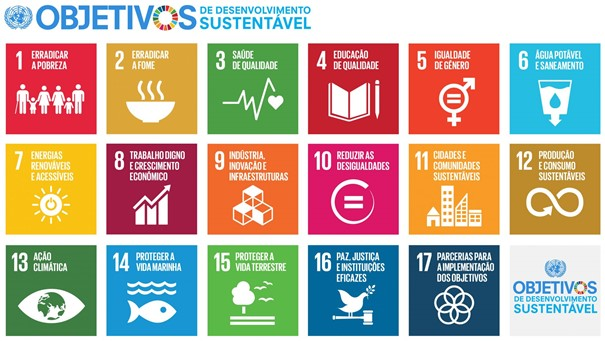
\includegraphics{Imagens/DesenvolvimentoSustentavel.jpg}
    \caption{Deve aparecer por baixo da figura. Se a figura for feita pelo aluno não necessita de referência. Caso seja retirada de uma fonte bibliográfica deve ser pedida autorização para a sua reprodução/cópia. Caso seja retirada de um website \textit{freevector} deve ser creditada de acordo com as regras estipuladas no mesmo. Por exemplo pode encontrar todos os ODS com reprodução livre em \href{URL}{https://www.un.org/sustainabledevelopment/news/communications-material/}}
    \label{fig:ODS}
\end{figure}

\begin{figure}[H]
\centering
\begin{subfigure}{.5\textwidth}
  \centering
  
\includegraphics[width=.6\linewidth]{Imagens/FigA.png}
  \caption{Explicar o que é Fig A}
  \label{fig:sub1}
\end{subfigure}%
\begin{subfigure}{.5\textwidth}
  \centering
  
\includegraphics[width=.6\linewidth]{Imagens/FigB.png}
  \caption{Explicar o que é Fig B}
  \label{fig:sub2}
\end{subfigure}
\caption{Exemplo de duas imagens numa figura.}
\label{fig:test}
\end{figure}


\section{Objetivos e perguntas de investigação \label{se:objetivos}}

Foram aprovadas a nível europeu (2020), medidas de alteração aos serviços de sistema, que serão seguidas pelos Estados-Membros. Nesta dissertação far-se-á a aplicação dessas medidas, identificando as melhorias face ao desenho actual e, avaliando se as novas medidas serão suficientes para assegurar a operação de um sistema eléctrico ~100\% renovável, eventualmente identificando acções adicionais que garantam a robustez e segurança do sistema eléctrico sem recurso a combustíveis fósseis.

\begin{description}
  \item[a)]\noindent É positivo para as vRES participar no mercado de reserva?
  \item[b)]\noindent Como configurar essa participação para optimizar o lucro do ponto de vista das vRES?
  \item[c)]\noindent Essa participação é positiva para o sistema eléctrico num todo?
\end{description}

\section{Organização do documento \label{se:organização}}

Explicar a lógica da organização em termos do conteúdo de cada secção. Por exemplo, no capitulo \ref{ch:revisao} mostram-se os estudos referentes a…….Na secção \ref{se:objetivos} mostra-se…..Na secção \ref{se:enquadramento} apresentam-se …..Finalmente, no capitulo \ref{ch:conclusao} são respondidas as perguntas de investigação, descrevem-se as limitações do estudo e recomendam-se …..para estudos futuros.

%Quando recompilam, todas estas labels são hiperlinks que podem usar para "saltar" para a secção/Capitulo em questão.

